%%%%%%%%%%%%%%%%%%%%%%%%%%%%%%%%%%%%%%%%%%%%%%%%%%%%%%%%%%%%%%
%% LaTeX template for the science justification to be       %%
%%     submitted as part of a regular ALMA proposal.        %%
%% This template should also be used for a ToO, DDT, or     %%
%%     mm-VLBI ALMA proposal, but NOT for Large Programs    %%
%%     (these have a separate template with more sections)  %%
%%                                                          %%
%%                      ALMA Cycle 9                        %%
%%                                                          %%
%%%%%%%%%%%%%%%%%%%%%%%%%%%%%%%%%%%%%%%%%%%%%%%%%%%%%%%%%%%%%%

%%%%%%%%%%%%%%%%%%%%%%%%%%%%%%%%%%%%%%%%%%%%%%%%%%
%%%%% How to convert this document to PDF %%%%%%%%
%%%%%%%%%%%%%%%%%%%%%%%%%%%%%%%%%%%%%%%%%%%%%%%%%%

% If your figures are stored as PostScript files, you can use the 
% following commands to generate a PDF file of your proposal:

%% latex file.tex
%% dvips file.dvi
%% ps2pdf file.ps file.pdf 


% If your figures are PDF images or bitmap pictures in PNG, JPG, or GIF format,
% you can use the pdflatex command to generate a PDF file from this template
% (note, however, that the pdflatex command does not handle PostScript files):

% pdflatex file.tex

% Warnings: 
%           1. You must make sure that PDF output generated from this
%              template is complete both when displayed with a viewer 
%              (acroread, for example) and when printed on paper.
%              LaTeX installations vary greatly and therefore it might 
%              not be possible to get all proposals to come out 
%              correctly with a single text page layout. 
%              In some cases you will have to adjust the 
%              \topmargin=-7mm command in the template to center the 
%              text vertically in the page.  
%           2. The scientific justification, figures, tables, references,
%              and public outreach statement must all fit within the
%              4-page limit.
%           3. You are free to include colour images in your proposal justification.
%              Proposals are distributed to ALMA Review Panels and to distributed
%              peer review reviewers in electronic form.
%              However, the scientific content of the images should still remain
%              clear when displayed or printed in black and white.
%           4. This template is for regular, ToO, DDT, or mm-VLBI ALMA proposals,
%              but NOT for Large Programs: these have a separate template with
%              more sections, and is available from the ALMA Science Portal


%%%%%%%%%%%%%%%%%%%%%%%%%%%%%%%%%%%%%%%%%%%%%%
%%%%% Default format: 12pt single column %%%%%
%% 12pt is the minimum font size allowed !! %%
%% This applies to everything, including    %%
%% references, figure captions, and tables  %%
%% ==> Proposals not compliant to this will %%
%%     be rejected. See Section 5.3.1 in    %%
%%     the ALMA Proposer's Guide            %%
%%%%%%%%%%%%%%%%%%%%%%%%%%%%%%%%%%%%%%%%%%%%%%

\documentclass[12pt,a4paper]{article}  %% DO NOT CHANGE to 11pt or less !

\usepackage{graphics,graphicx}

%%%%%%%%%%%%%%%%%%%%%%%%%%%%
%%%%%% Page dimensions %%%%%
%%%%%%  DO NOT CHANGE  %%%%%
%%%%%%%%%%%%%%%%%%%%%%%%%%%%

\textheight=247mm
\textwidth=180mm
\topmargin=-7mm
\oddsidemargin=-10mm
\evensidemargin=-10mm
\parindent 10pt

%%%%%%%%%%%%%%%%%%%%%%%%%%%%%
%%%%% Start of document %%%%% 
%%%%%%%%%%%%%%%%%%%%%%%%%%%%%

\begin{document}
\pagestyle{plain}
\pagenumbering{arabic}
 
% The title, abstract and list of investigators should NOT be included in the
% Scientific justification. The title and abstract are put automatically on the cover page.

%%%%%%%%%%%%%%%%%%%%%%%%%%%%%%%%%%%%%%%%%
%%%%% Body of science justification %%%%%
%%%%%%%%%%%%%%%%%%%%%%%%%%%%%%%%%%%%%%%%%

%% ENTER TEXT, FIGURES AND TABLES BELOW
%% Minimum font size for all text, references, figure captions, and tables is 12pt
%% Proposals not compliant to this will be rejected. See Section 5.3.1 in the ALMA Proposer's Guide.

\section{Scientific justification}

% ALMA uses two systems to review the proposals submitted in the Main Call.
% All proposals requesting less than 50 h on the 12-m Array and all ACA stand-alone proposals requesting less
% than 150 h on the 7-m Array will be reviewed by Distributed peer review (see Section 1.2.1 of the Proposer's Guide).
% All Large Programs will be reviewed by Panels. 
% Additionally, both systems will follow a dual-anonymous procedure, in which the proposers do not know
% who are the reviewers and the reviews do not who are the proposers.
%
% Please refer to the guidelines before writing your proposal:
%     https://almascience.org/proposing/alma-proposal-review/dual-anonymous
%
% In the following part, describe the scientific background of the project,
% pertinent references and previous work relevant to this 
% proposal, together with any figures and tables that you judge necessary
% (use the following two examples as templates, or remove)
% Please do not disclose the name(s) of the proposer(s), and write the proposal in a way
% such that the proposer(s) cannot be identified. 
 
%-----------------------------Figure Start---------------------------

% The 'scale' parameter below allows you to scale the figure so that it fits within the page.
% In this case the figure was scaled to 20% of its original size.
% Note: for .png files one has to use pdflatex, not classic latex
%
% Minimum font size for references: 12pt 
% Proposals not compliant to this will be rejected. See Section 5.3.1 in the ALMA Proposer's Guide.

\begin{figure}[tbh]
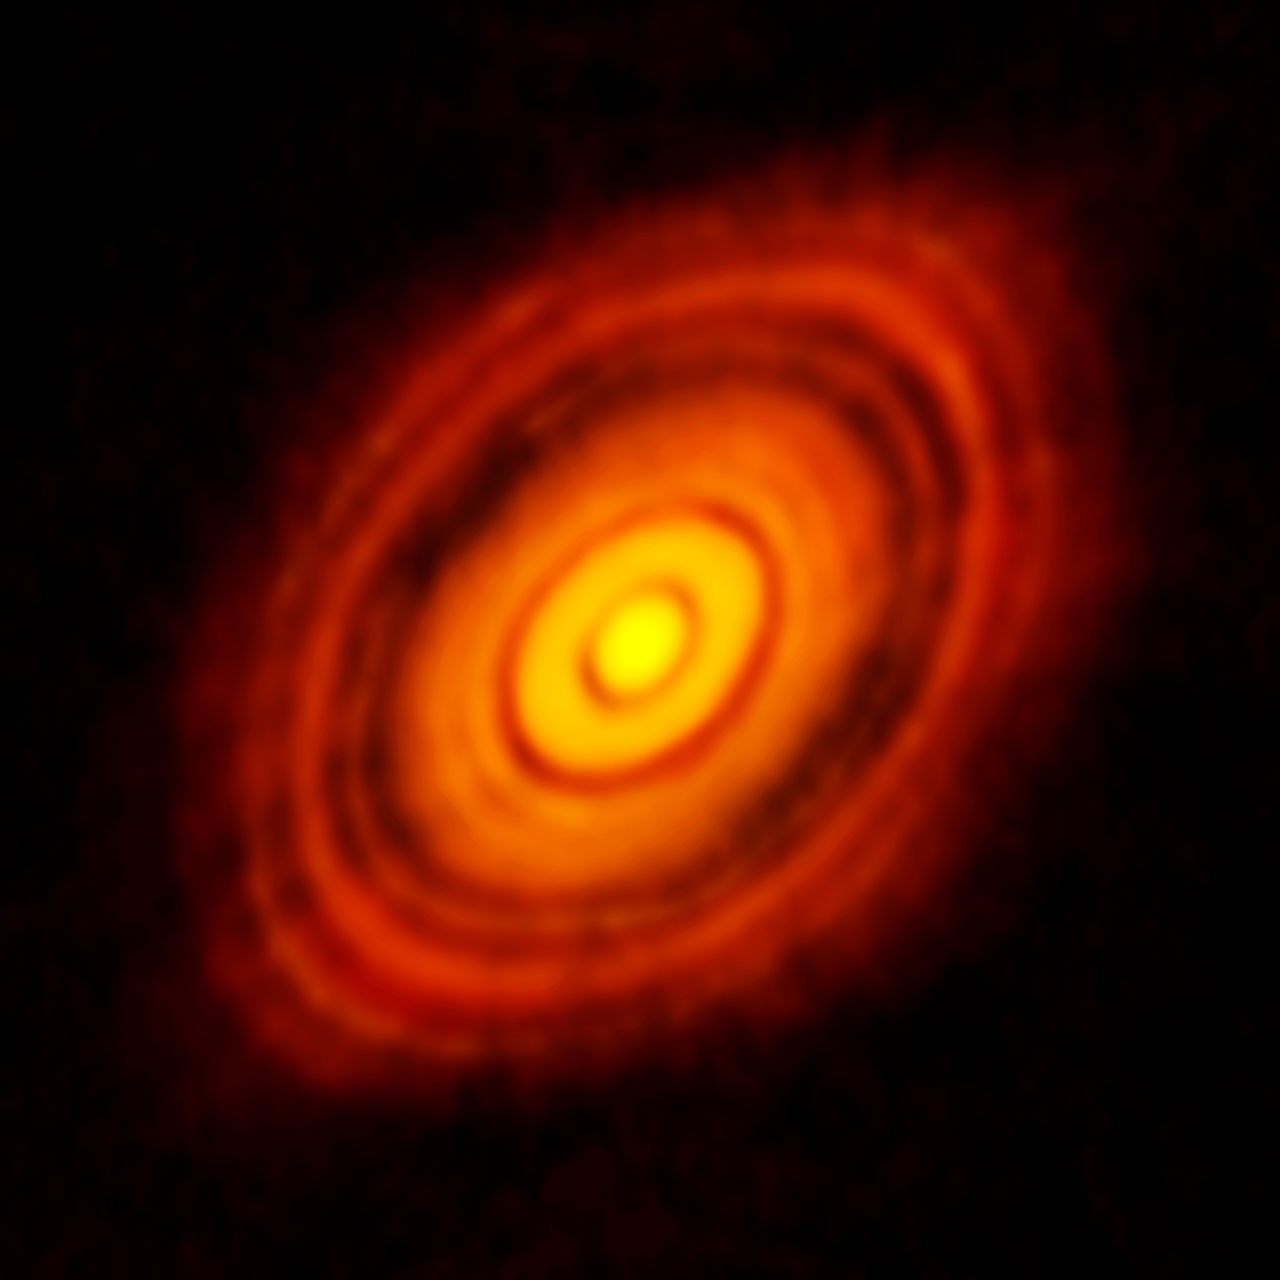
\includegraphics[scale=0.2]{HL_tau.jpg}
\caption{\em{ALMA image of the protoplanetary disc surrounding the young star HL Tauri.}}
\end{figure}
%-----------------------------Figure End------------------------------

%-----------------------------Table Start-----------------------------

% Minimum font size for references: 12pt 
% Proposals not compliant to this will be rejected. See Section 5.3.1 in the ALMA Proposer's Guide.

\begin{table}[tbh]
\begin{center}
\caption[]{\em{Here we show the continuum sensitivity required per band.}}
\begin{tabular}{cc}
\hline \noalign {\smallskip}
Frequency (GHz) & Sensitivity (mJy) \\
\hline \noalign {\smallskip}
300 & 0.10 \\
850 & 0.50 \\
\hline \noalign {\smallskip}
\end{tabular}
\end{center}
\end{table}
%-----------------------------Table End ------------------------------

\section{Description of observations}

% Please describe the observations to be made and their specific
% purpose, with a clear explanation of the need for, and 
% appropriateness of, ALMA Cycle 9 data.  


\section{References}

% List references here
% Minimum font size for references: 12pt 
% Proposals not compliant to this will be rejected. See Section 5.3.1 in the ALMA Proposer's Guide.

\noindent [1] Author1 et al. year, journal, vol, page

\noindent [2] Author2 et al. year, journal, vol, page


%%%%%%%%%%%%%%%%%%%%%%%%%%%
%%%%% End of document %%%%%
%%%%%%%%%%%%%%%%%%%%%%%%%%%

\end{document}

